
\begin{question}
\textbf{Draw} the polynomial function \(f(x)\) shown in factored and
expanded forms. Be sure to indicate the roots, where the function is
positive or negative, and end behavior.

\[f(x) = 3 \left(x - 4\right) \left(x - 3\right)^{2} \left(x + 2\right) \left(x + 5\right)\]

\[f(x) = 3 x^{5} - 9 x^{4} - 81 x^{3} + 285 x^{2} + 234 x - 1080 \]
\end{question}

\begin{solution}
You need to consider the roots and end behavior. If a root has even
multiplicity, you need to bounce the curve off the \(x\)-axis there.

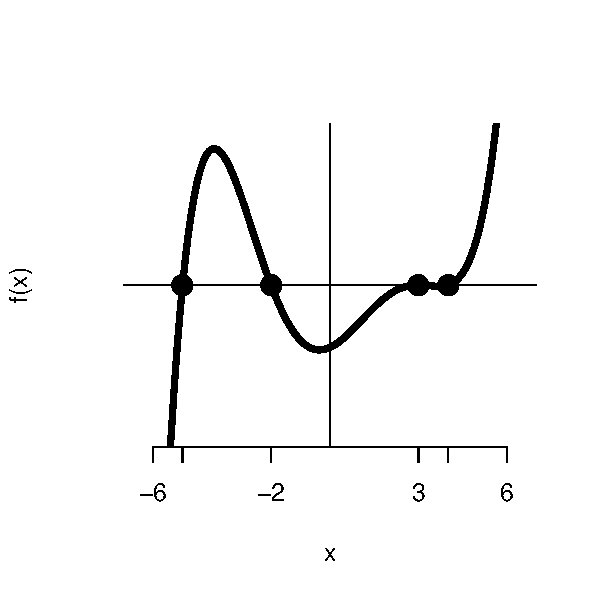
\includegraphics{unnamed-chunk-2-1-2.pdf}\\
\end{solution}

